\documentclass[border=4pt]{standalone}
\usepackage{tikz}
\usetikzlibrary{arrows.meta,positioning,fit,calc,backgrounds}
\usepackage[T1]{fontenc}
\usepackage{lmodern}
\usepackage{amsmath,amssymb}
\definecolor{wsp}{HTML}{2A78D6}
\definecolor{dflt}{HTML}{7A7974}
\definecolor{trn}{HTML}{EB6834}
\definecolor{sb}{HTML}{1BAF7A}
\definecolor{look}{HTML}{6250D6}
\definecolor{ink}{HTML}{0B0B0B}
\definecolor{ink2}{HTML}{52514E}
\definecolor{paper}{HTML}{F4F3EF}
\tikzset{
  box/.style={draw=ink2, rounded corners=3pt, fill=paper, align=center, inner sep=5pt, font=\small, text width=#1},
  box/.default=3.0cm,
  hl/.style={draw=wsp, line width=0.9pt, fill=wsp!8},
  arr/.style={-{Stealth[length=2.2mm]}, line width=0.7pt, draw=ink2},
  note/.style={font=\footnotesize\itshape, text=ink2, align=center},
}

\begin{document}
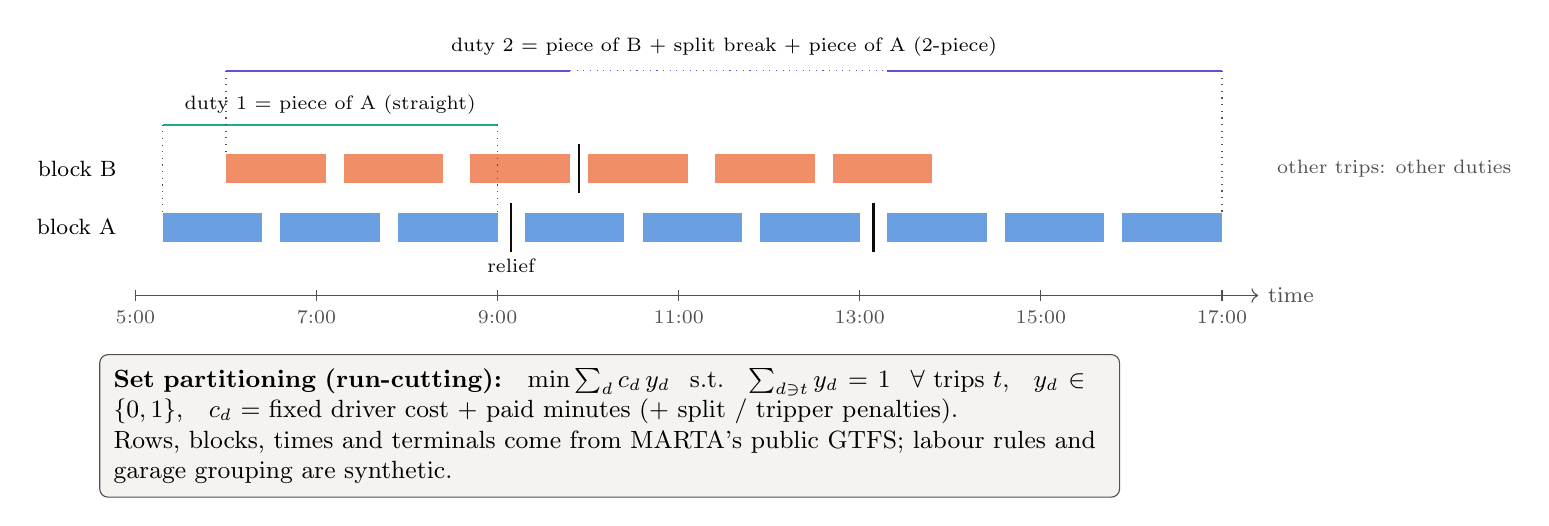
\begin{tikzpicture}[x=1.15cm,y=0.62cm]
% time axis
\draw[ink2,->] (0,0) -- (12.4,0) node[right,font=\footnotesize]{time};
\foreach \h/\l in {0/5:00,2/7:00,4/9:00,6/11:00,8/13:00,10/15:00,12/17:00}{\draw[ink2] (\h,0.12)--(\h,-0.12) node[below,font=\scriptsize]{\l};}
% block 1 trips
\node[font=\footnotesize,anchor=east] at (-0.1,1.4) {block A};
\foreach \a/\b in {0.3/1.4,1.6/2.7,2.9/4.0,4.3/5.4,5.6/6.7,6.9/8.0,8.3/9.4,9.6/10.7,10.9/12.0}{\fill[wsp!70] (\a,1.1) rectangle (\b,1.7);}
\node[font=\footnotesize,anchor=east] at (-0.1,2.6) {block B};
\foreach \a/\b in {1.0/2.1,2.3/3.4,3.7/4.8,5.0/6.1,6.4/7.5,7.7/8.8}{\fill[trn!75] (\a,2.3) rectangle (\b,2.9);}
% relief points
\foreach \x in {4.15,8.15}{\draw[ink,line width=0.9pt] (\x,0.9)--(\x,1.9);}
\node[font=\scriptsize,ink] at (4.15,0.6) {relief};
% duties
\draw[line width=0.8pt,sb] (0.3,3.5) -- (4.0,3.5) node[midway,above,font=\scriptsize,text=ink]{duty 1 = piece of A (straight)};
\draw[line width=0.8pt,look] (1.0,4.6) -- (4.8,4.6);
\draw[line width=0.8pt,look] (8.3,4.6) -- (12.0,4.6);
\draw[look,dotted] (4.8,4.6) -- (8.3,4.6);
\node[font=\scriptsize,above] at (6.5,4.7) {duty 2 = piece of B + split break + piece of A (2-piece)};
\draw[ink2,dotted] (1.0,4.6)--(1.0,2.9); \draw[ink2,dotted] (12.0,4.6)--(12.0,1.7);
\draw[ink,line width=0.9pt] (4.9,2.1)--(4.9,3.1);
\node[font=\scriptsize,text=ink2,anchor=west] at (12.5,2.6) {other trips: other duties};
\draw[ink2,dotted] (0.3,3.5)--(0.3,1.7); \draw[ink2,dotted] (4.0,3.5)--(4.0,1.7);
% model
\node[box=12.6cm, anchor=north west, align=left] at (-0.4,-1.2) {\textbf{Set partitioning (run-cutting):}\quad
$\min \sum_{d} c_d\, y_d \;\;\text{s.t.}\;\; \sum_{d \ni t} y_d = 1 \;\;\forall \text{ trips } t,\;\; y_d\in\{0,1\}$,\quad
$c_d$ = fixed driver cost + paid minutes (+ split / tripper penalties).\\
Rows, blocks, times and terminals come from MARTA's public GTFS; labour rules and garage grouping are synthetic.};
\end{tikzpicture}
\end{document}
